%%%%%%%%%%%%%%%%%%%%
\chapter{Comparison and Results}
\label{cha:ComparisonAndResults}

This chapter presents the results that are achieved in the development of the FM Radio Receiver project, with the chosen different methods.
However, the main focus is to compare the results that are achieved with HLS and VHDL, since these are the major implementation variants of the project.

%%%%%%%%%%%%%%%%%%%%%%%%%%%%%%%%%%%%%%%%%%%%%%%%%%%%%%%%%%%%%%%%%%%%%%%%%%%%%%
\section{General}

A main objective of this thesis is to implement an FM radio receiver in multiple different methods.
This includes GNU Radio, Matlab, VHDL and HLS, which all have their advantages and disadvantages and surface different challenges to the developer.
The target functionality is to listen to the audio broadcast signal of an FM radio station.\\

All of the listed methods are implemented and the target functionality is achieved with all of them.
However, the level of detail that is required in the implementation, and the resulting effort and time it takes to implement the respective variant, differs by a large factor.
This is mainly due to the different levels of abstraction, so that the low-level algorithms do not need to be known.\\

In the following sections, especially the HLS and VHDL implementations are compared on the basis of metrics, but also based on the experience during development.


%%%%%%%%%%%%%%%%%%%%%%%%%%%%%%%%%%%%%%%%%%%%%%%%%%%%%%%%%%%%%%%%%%%%%%%%%%%%%%
\section{Functionality}

Generally, both tools -- HLS and VHDL -- provide the capabilities to implement any functionality in one or the other method.
However, the implementation is done in a different level.
VHDL uses an approach that is very close to the hardware, such as clock cycles and flipflops, while HLS describes the logic on an algorithmic level.\\

The implementation is split into two main parts, the communication interfaces and the DSP.
The results are presented in the following sections.

% Functionality same?
% DSP yes, AXI no (FSM of axi-stream)
% unit tests

%%%%%%%%%%%%%%%%%%%%%%%%%%%%%%%%%%%%%
\subsection{Interfaces}

The AXI4-Lite memory-mapped bus is implemented to have an exactly equal behaviour in both variants.
There are read-only and read-writeable registers, which are all mapped onto a single base address.\\

The AXI stream interface however does not show the exact same behaviour.
Here, the HLS variant is using the AXI stream according to its protocol, while the VHDL variant is implemented differently.
It uses a simplified logic for the ready-flag, which reduces the effort in implementation.
However, from the perspective of the communicating blocks, the interface is usable like a regular AXI stream.
The implementation details are explained in Section~\ref{sec:impl:vhdl:interfaces}.\\

In the final, integrated system on the SoC hardware, the CPU is able to communicate with both IPs via their interfaces successfully.
Status and configuration data can be read and written through the AXI4-Lite interface, and the streaming data for the DSP chain is successfully sent through the AXI streams as well.

%%%%%%%%%%%%%%%%%%%%%%%%%%%%%%%%%%%%%
\subsection{Audio Output}

The audio output of the HLS and VHDL variants is compared with the Matlab model, which serves as the reference.
Additionally, the results of the testbench are compared with their respective result in the actual hardware.
In summary, it can be stated that the DSP chain produces a very similar audio output in all the compared data sets.
However, differences remain, which are presented in the following paragraphs and diagrams.

\includepicture [1.0] [0] {Comparison of the IP audio output signals, in simulation and hardware, against the Matlab model. The HLS variant matches the model, while the VHDL output diverts by a certain amount. Also, VHDL differs between simulation- and hardware results.} {audio_output_compare_tb_vs_hw} {img/matlab/audio_output_compare_tb_vs_hw}

%%%%%
\subsubsection{Comparing against the Matlab reference}

In the comparison against the Matlab model, the HLS variant achieves a very exact match of the output signal.
However, the VHDL implementation differs by a certain amount.
There seems to be an issue in the signal separation between the left and right audio channels.
This is visible in the analysis of the audio signal, as shown is Figure~\ref{fig:audio_output_compare_tb_vs_hw}.
The signal strength of the left channel in the upper diagram is weaker than expected, while the right channel in the lower diagram is stronger.
This imbalance can also be observed by listening to the audio output via speakers.\\

The cause for this issue may be located in several components in the design.
This includes the FM demodulator, the carrier recovery, i.e. the 38~kHz carrier, as well as a sample timing shift in the final summation and substraction to recover the left and right channels.
The FIR filter has a successfully passing unit test and is thus assumed to be correct.
Also the fixed point data type with its overflow- and rounding behaviour is suspected to be a potential issue.
Due to the time limitation in the elaboration of this thesis, this issue can not be traced down to the root cause and thus still persists in the current implementation.
However, from the system-level point of view of this thesis, the IP works and can be integrated into the final system.

%\includepicture [1.0] [0] {Comparison of the IP audio output signals against the Matlab model. The HLS variant matches the model, while the VHDL output diverts by a certain amount.} {audio_output_compare_ips_vs_matlab} {img/matlab/audio_output_compare_ips_vs_matlab}

%%%%%
\subsubsection{Comparing simulation- against hardware results}

Here, the results of the simulation testbenches are compared against the values that are read from the FPGA directly.
Ideally, the values should be exactly the same.
However, Figure~\ref{fig:audio_output_compare_tb_vs_hw} shows that this is not always the case.
Again, the HLS implementation does have a matching result, whereas the VHDL variant has deviating values.
The explanation here may be linked with above suspicions, but may also be linked to the initial reset values that exist in the hardware.
In the HLS implementation, the reset logic of several registers is implemented automatically, whereas in VHDL these conditions need to be implemented manually.
Therefore, the IPs internal state, i.e. the register values, may be different at the beginning, which leads to an error propagation throughout the design.
The entire DSP chain is built like a pipeline and therefor it takes a number of samples to process, before the 'wrong' intermediate values are flushed out.
All that may be the cause for the deviating values in the VHDL design.\\

Again, the time limitation in the elaboration of this thesis does not allow a deeper analysis and investigation of this issue.
However, the end-to-end system design enables the developer to analyze an issue like this in a convenient way, in quick iterations.
Any adaptions in the VHDL design can be simulated and integrated into the FPGA with automated scripts.
Both results can then be analyzed and compared, which may lead to further adaptions.\\


%%%%%%%%%%%%%%%%%%%%%%%%%%%%%%%%%%%%%%%%%%%%%%%%%%%%%%%%%%%%%%%%%%%%%%%%%%%%%%
\section{Code Development}

In the development of a software project, the metric for the lines of code can be used to give an idea of the scale, or volume of the project.
The time it takes to implement a certain set of features can also give such an insight and a hint of the project's complexity.
It is a subjective metric though, since it is heavily influenced by the respective developer's experience in the specific application.
However, both metrics are applied to the FM Radio Receiver project.\\

At this point, it is important to note that the results that are presented in this section are very specific to the chosen architecture, testbench framework, and the implementation style generally.
Therefore, the numbers that are presented here may vary widely by modifying any of these factors, i.e. using a different testbench framework for VHDL.
Thus, a generalization in the art of \textit{HLS always requires less code than VHDL} can not be stated.
However, the results in this section can give an idea and overview of this topic and provide a detailed comparison for this specific project.

%%%%%%%%%%%%%%%%%%%%%%%%%%%%%%%%%%%%%
\subsection{Lines of Code}

Several parts of the system design are taken into account to analyze the lines of code, to give an impression over the largest code parts in the project.
Figure~\ref{fig:lines_of_code_pie_charts} shows multiple pie charts, which represent the proportions of the lines of code in the respective system design parts.
Table~\ref{tab:lines_of_code} displays the actual numbers of code lines, to quantify the size of the respective parts.\\

Interesting details can be found by analyzing these charts.
The upper chart shows that the implementation of the hardware support, in the form of Vivado project scripts and the \cplusplus\ application software, takes a large part of the code with 27\%.
The remaining majority of the code belongs to the development of the IPs.
This includes the implementation of the Matlab model, the VHDL and HLS code, as well as the common testbench.
The chart also reveals that the VHDL implementation with its accompanying testbench requires more than twice the amount of code compared to the HLS version, i.e. 32\% versus 14\%.\\

The lower charts highlight several differences between HLS and VHDL.
Specifically, the code proportions between IP design and testbench are pointed out.
The charts show that HLS requires about the same amount of code for IP design and testbench.
VHDL requires the largest part of code in the IP design, while the testbench code amount is relatively small.
It is to be noted, that the common testbench consists of 4\%, which equals 630 lines of Python code.
Therefor, the testbench code of both IPs is relatively small, because the entire analysis part is shared.

\begin{figure}%
  \centering
  \subfloat[\centering Overview of the proportions between all the implemented code parts of the entire project.]{{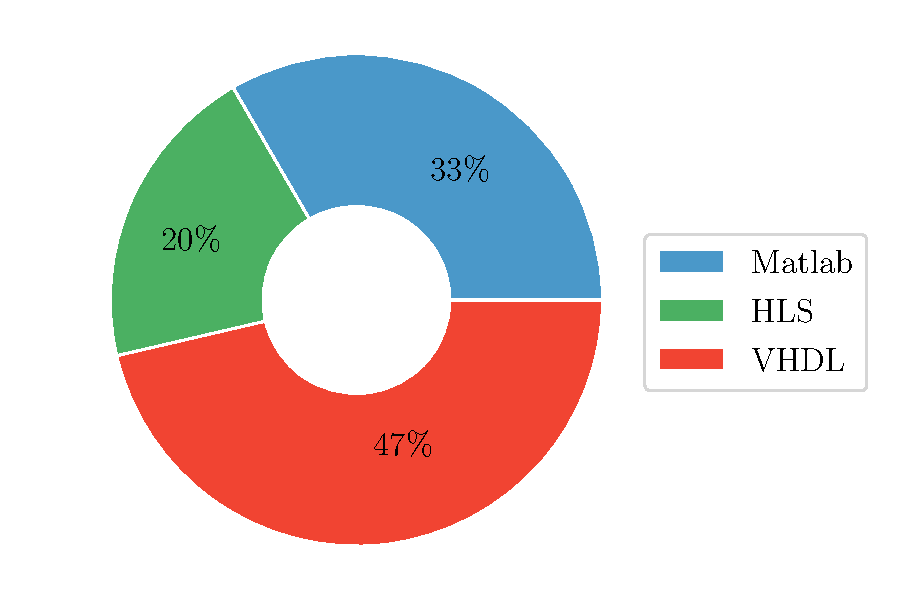
\includegraphics[trim=10 40 10 10,clip, width=0.65\textwidth]{img/matlab/lines_of_code_pie_chart_py_all} }}%
  \\
  %\hspace{\fill}
  \subfloat[\centering HLS in detail.]{{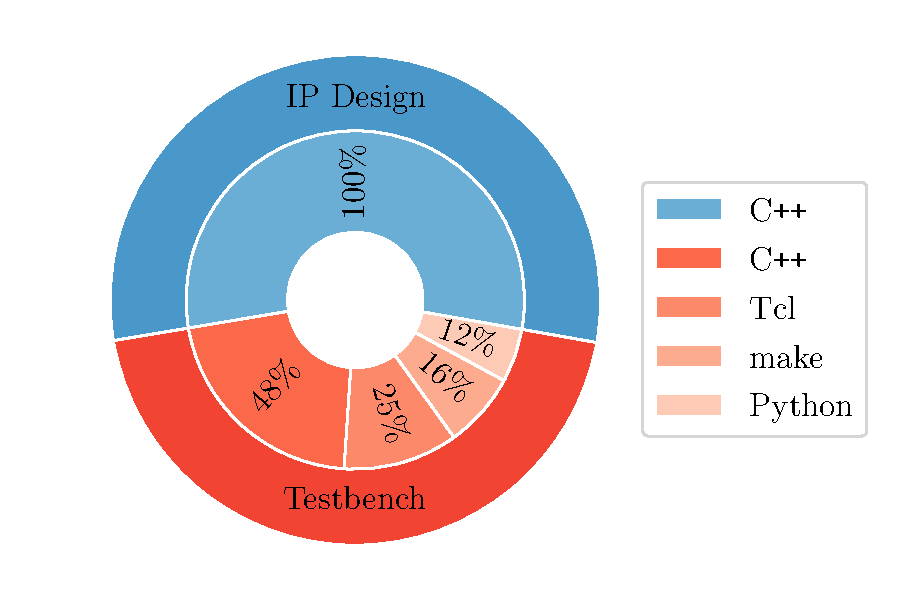
\includegraphics[trim=10 10 10 10,clip, width=0.49\textwidth]{img/matlab/lines_of_code_pie_chart_py_hls} }}%
  %\hspace{\fill}
  %\vspace{3cm}
  \subfloat[\centering VHDL in detail.]{{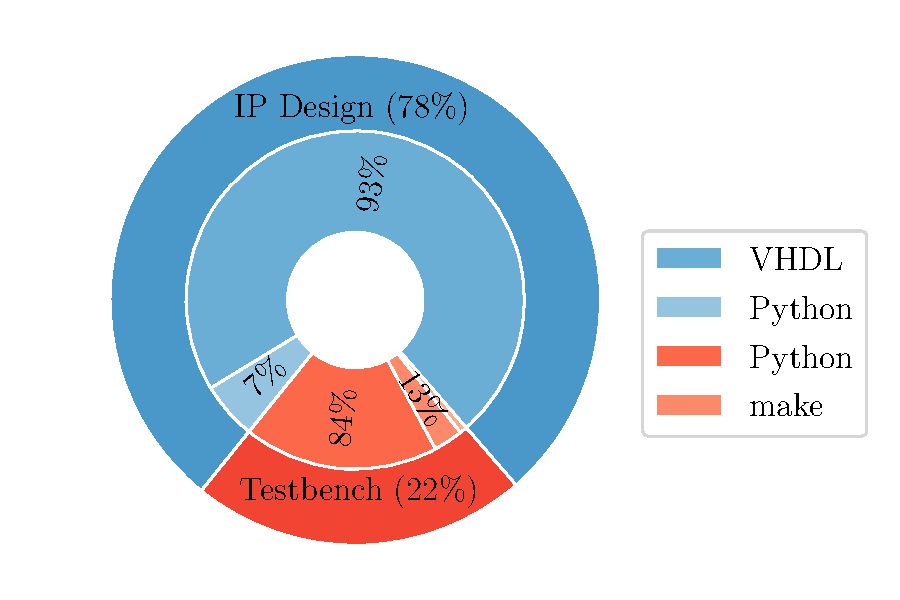
\includegraphics[trim=10 10 10 10,clip, width=0.49\textwidth]{img/matlab/lines_of_code_pie_chart_py_vhdl} }}%

  \caption{Lines of code of the respective code parts in the entire project, presented in multiple pie charts. The percentages of code in IP design and testbench for the HLS and VHDL implementations are shown in detail in the lower diagrams.}%
  \label{fig:lines_of_code_pie_charts}%
\end{figure}

\begin{table}[]
  \centering
  \begin{tabular}{l|c|c|}
  \cline{2-3}
  \textbf{}                                     & \multicolumn{1}{r|}{\textbf{IP Design}} & \multicolumn{1}{l|}{\textbf{Testbench}} \\ \hline
  \multicolumn{1}{|l|}{VHDL}                 & 3000                                    & 850                                     \\ \hline
  \multicolumn{1}{|l|}{HLS}                  & 920                                     & 740                                     \\ \hline
  \multicolumn{1}{|l|}{Common Testbench}        & \multicolumn{2}{c|}{630}                                                          \\ \hline
  \multicolumn{1}{|l|}{Matlab Model}            & \multicolumn{2}{c|}{2730}                                                         \\ \hline
  \multicolumn{1}{|l|}{Vivado Scripts}          & \multicolumn{2}{c|}{490}                                                          \\ \hline
  \multicolumn{1}{|l|}{\cplusplus\ Application} & \multicolumn{2}{c|}{2800}                                                         \\ \hline
  \end{tabular}
  \caption{The actual number of code lines for each code part, split in IP design and testbench, where applicable. All numbers are rounded up to tens.}
  \label{tab:lines_of_code}
\end{table}


%%%%%%%%%%%%%%%%%%%%%%%%%%%%%%%%%%%%%
\subsection{Implementation Time}

The metric of implementation time -- the time it takes to implement a specific feature -- is a subjective measure, since it heavily depends on the respective developer's experience, as already noted above.
In the present case, there is a strong background of knowledge and practical experience in VHDL design, while there is only very little of such in HLS design.
However, this metric is used in this section to specifically compare HLS with VHDL in this project.
Certain features are chosen for this comparison and their implementation times were logged during the actual implementation process.
The implementation is always considered as the HDL description, including the corresponding testbench code, to verify the respective correct functionality.
Table~\ref{tab:implementation_time_logging} shows the direct comparison between HLS and VHDL implementation times for these features.\\

\begin{table}[]
  \centering
  \begin{tabular}{l|c|c|}
  \cline{2-3}
                                                   & \multicolumn{2}{c|}{\textbf{Time [h]}} \\ \hline
  \multicolumn{1}{|l|}{\textbf{Feature}}           & \textbf{HLS}      & \textbf{VHDL}      \\ \hline
  \multicolumn{1}{|l|}{AXI Stream Interface}       & 8                 & 12                 \\ \hline
  \multicolumn{1}{|l|}{AXI4-Lite Interface}        & 2                 & 10                 \\ \hline
  \multicolumn{1}{|l|}{LED Control Register}       & 1                 & 2                  \\ \hline
  \multicolumn{1}{|l|}{Build Information Register} & 8                 & 5                  \\ \hline
  \multicolumn{1}{|l|}{Pass-Through Mode Register} & 1                 & 1                  \\ \hline
  \multicolumn{1}{|l|}{FIR Filter}                 & 13                & 7                  \\ \hline
  \multicolumn{1}{|l|}{Sample Decimation}          & 15                & 1                  \\ \hline
  \multicolumn{1}{|l|}{Receiver Structure}         & 13                & 33                 \\ \hline
  \multicolumn{1}{|l|}{\textbf{Sum}}               & \textbf{61}       & \textbf{71}        \\ \hline
  \end{tabular}
  \caption{Implementation time logging for a specific set of features, for the direct comparison between HLS and VHDL.}
  \label{tab:implementation_time_logging}
\end{table}

The following paragraphs present an insight into how the implementation times of the listed code parts arise.

%%%%%%%%%%%%%%%%%%%%%%%
\subsubsection{AXI Stream Inferface}

This is the main interface for the data input and -output of the DSP chain.
In HLS it can be automatically inferred by adding pragma directives to the respective function parameter variables.
Also the testbench code is implemented like a regular function call.
Therefore, the actual interface logic is completely hidden from the developer.
In VHDL on the other hand, this logic has to be implemented manually.
Also the testbench has to be hooked up with the correct signals and have a verificator logic, that supports the functional verification of an AXI stream interface.
Otherwise, this logic would have to be implemented manually as well.
In the time comparison, the larger amount of manual implementation in VHDL is clearly visible.
It is to note that this comparison does not compare functionally equivalent implementations, because the actually implemented logic in VHDL does not use the ready-flag correctly, as explained in the previous chapters.
According to this fact, a further increase in implementation hours should actually be considered for VHDL.
However, also the HLS implementation has its particular characteristics that need to be understood for a fully functional implementation.
Following the respective user guides and implementation examples provides a good starting point for that.

%%%%%%%%%%%%%%%%%%%%%%%
\subsubsection{AXI4-Lite Interface}

This interface is used to control IP settings and to read status information.
Similar to the previous AXI Stream interface, also this AXI4-Lite memory-mapped interface is automatically generated by HLS, while this has to be done manually in VHDL.
To create this process more efficiently and extendable, a Python script is used, which can also automatically generate VHDL code for the registers' memory map.
This turns out to be a multiplicator in productivity for the implementation of registers.
The register generator script was previously used in projects and is therefor already well-known and tested before it is used in this project.
However, the VHDL code only represents one part of the interface -- the second part is the firmware driver that is used in the application software.
Even though the register generator script also generates a \cplusplus\ header file that includes several address offset definitions of the registers, the actual driver functions need to be implemented manually.
Several files need to be integrated into a pre-defined folder structure, in order to enable a correct integration of the IP in a Vivado block diagram.\\

Again, the amount of manual steps in the VHDL implementation are clearly represented in the number of hours that are spent.

% TODO: mention figure out of read-only and read-write types (pointer/reference)
% TODO: mention testbench (vhdl: support block, hls: simple access to variable)

%%%%%%%%%%%%%%%%%%%%%%%
\subsubsection{Registers}

Once the AXI4-Lite memory-mapped interface's main functionality is implemented, further registers can be added.
In the specific implementation for this project, registers for LED control, the DSP mode, as well as a build information register are added.
The latter holds information about the build date and -time of the IPs, and is particularly time-consuming because of the implementation of the respective drivers to convert the date format in both variants.
In contrast, the addition of the LED control and DSP mode registers is simple and fast, because of the auto-generated code in HLS and VHDL with usage of the register engine.
The single bits in the LED control register directly represent the LEDs' values on the hardware.
The DSP mode register can select the regular FM radio mode and a pass-through mode, which simply forwards the streaming data without any processing.
Summing up, the addition of registers to the design can be time-consuming in both variants, depending on the required driver functionality.
However, the general tendency is that VHDL requires more time, because of this driver issue.

%%%%%%%%%%%%%%%%%%%%%%%
\subsubsection{FIR Filter}

The FIR filter is one of the main DSP blocks of the design, as it is used in multiple instances throughout the design.
Therefore, its implementation was done with special care, in order to guarantee its correct functionality.
Consequently, a unit test is implemented in the testbench, which is also included in the listed number of implementation hours.\\

For the \cplusplus\ version, a code example for an FIR filter, which is provided by Xilinx HLS, is taken and modified for the present purpose.
The VHDL variant is taken from an older DSP project, which was previously developed during a university course.
However, the integration and testbench code is developed for this project, specifically.
Here, the HLS implementation took significantly longer, because of the limited knowledge regarding the usage of an AXI stream interface.
It is the first time in the project, that this type of interface is applied in the IP design and used in the testbench.
The VHDL implementation was straightforward in comparison.
The testbenches compare the FIR filters' output with the Matlab model's pilot tone output.
Both variants match the output results of the Matlab model successfully.

%%%%%%%%%%%%%%%%%%%%%%%
\subsubsection{Sample Decimation}

The implementation of the sample decimation functionality differs slightly between the two variants, HLS and VHDL.
This is explained in Section~\ref{sec:impl:hls:sample_rate_reduction}.
The implementation time of the HLS version is severely larger than the VHDL version.
This is mainly due to the limited knowledge of the functionality of the AXI stream interface at this stage in the project's implementation, just as previously mentioned with the FIR filter.
The initial version was implemented like the VHDL version -- a counter that only triggers the subsequent DSP blocks upon a certain number of samples was received.
However, this led to an endlessly blocking AXI stream in the testbench execution.
The reason was, that the read-function can only read a sample when the respective stream contains a sample, and that it is a blocking function.
Because the sample decimator did not write a sample every time, the subsequent read-function blocked indefinitely.
A thorough investigation in several user guides, in combination with step-by-step debugging, the issue was found and led to the current, working implementation, which processes a number of samples, before it forwards one sample.
The process of finding this issue explains the largely varying implementation times, as listed in Table~\ref{tab:implementation_time_logging}.

%%%%%%%%%%%%%%%%%%%%%%%
\subsubsection{Receiver Structure}

The implementation of the receiver structure requires the combination of several previously implemented blocks, such as the FIR filter and any interfaces.
This is done according to the Matlab model, to resemble its functionality.
The VHDL version is significantly more time consuming in comparison to HLS.
However, it is to note at this point that the VHDL version is implemented first, and thus some issues are already solved by the time of the HLS implementation.
Nevertheless, the VHDL implementation takes longer, as it requires more detailed care in the signal level.
This specifically includes the clock-alignment of any signals that need to be used in a combination.
For example, if two parallel FIR filters produce output signals that are to be added, they need to be aligned so that they are valid at the time of the summation.
This often requires analysis and debugging in a signal wave form.
In HLS this is not required, since the validity of a signal is determined internally by the HLS compiler, according to the usage of the respective data variables.
Another factor that adds up to the implementation time is the number of lines of code, as presented in Table~\ref{tab:lines_of_code}.
The VHDL IP design requires 3000 lines, while the HLS IP design only takes 920 for the same functionality.
Again, this is a subjective measure -- several factors such as code style, or the developer's experience play a role -- but still shows a good representation of the implementation effort for this project.\\

In the final summation over several implementation times of all the listed features, the two variants HLS and VHDL only differ by 10 hours, which is around 15\%.
However, as the previous paragraphs explain, prior knowledge regarding HLS was limited and had to be gathered during the ongoing implementation.
Nevertheless, even consiering this fact, the HLS implementation is faster than the VHDL equivalent.
Thus, with an equal amount of prior knowledge and experience, it is assumed that an HLS implementation can lead to a successfully functioning result significantly faster.


% Implementation effort/time
%    -- see logged times; is subjective; had no previous knowledge
%    -- AXI interfaces --> huge effort in VHDL...
%        (mention Johannes Walter for generously providing/allowing the Register Engine script, adapted for this thesis)
%    -- drivers are auto-generated with HLS! huge time-saving..
%       (maybe show the code of AXI4-Lite interface and its generated driver
%        --> difference between R/W and RO!;
%        and show screenshots of the IP in the block design)

% Issues
% -- HLS Debug Error with Bitwidth:
%       Not sure what the error was.
%       Parallel delay for I/Q didn't work.
%       The order of every 2nd data value was wrong.
%       Using a single delay fixed it.
% -- HLS driver generation
%       Fixing issue with auto-generated driver.
%       It did not get imported into the SDK.
%       Problem was that HLS project and top-level
%       did not have the same name....

%%%%%%%%%%%%%%%%%%%%%%%%%%%%%%%%%%%%%%%%%%%%%%%%%%%%%%%%%%%%%%%%%%%%%%%%%%%%%%
\section{Simulation Speed}

In this section, the simulation speed of the multiple implementation variants in their various abstraction levels are compared.
Simulation speed in this context refers to the number of input samples that the DUT can process in a time unit, like one second.
In the current application, the antenna signal is recorded and replayed to the DUT in the simulation.
This ensures a reproducable result, so that the different variants can be compared against each other reliably.\\

Figure~\ref{fig:impl_time_analysis} shows this direct comparison of processed samples per second for the implementation variants.
The measurements always include the testbench setup-phase, and the run-phase.
The setup-phase mainly consists of loading the recorded data and its preparation, so that it can be fed into the DUT.
The run-phase then actually applies this test data to the DUT and stores the respective output results.
All time measurements are taken without the result analysis, since this is the exact same, shared code between all variants and thus takes the same amount of time everywhere.
Several measurements are done multiple times, to achieve an average result, that is independent of the current processor load of the host PC.\\

The diagram shows an immense difference of simulation speed between the variants.
It is important to note that the y-axis has a logarithmic scale, as a method to enable the presentation of the values in multiple orders of magnitude.
VHDL only achieves around 20 samples per second.
This is by far the slowest method, which is expected because of the way of how VHDL is simulated.
This can not be explained in detail here, but one main feature of a VHDL simulator is its capability to simulate parallel processes, as they occur in actual parallel hardware.
The VHDL simulator therefor needs to evaluate several concurrent processes and statements, whenever any of the interacting signals change their value, and this is time-consuming.
In the current case, there is an additional interface between the VHDL simulator and the Python testbench framework, which likely additionally slows down the simulation.
The HLS testbench in comparison achieves around 50000 samples per second, which is a speed-up factor of 2500.
This is specifically talking about the HLS C/\cplusplus-simulation.
The main reason for the speed-up therefor is, that in this type of simulation no timing behaviour is simulated -- any processes are treated as C/\cplusplus\ functions that runs like a regular executable on the host CPU.
Also, the HLS compiler is using native \cplusplus\ data types to represent the signals, where possible, which results in the faster execution of the code.
Finally, the simulation in Matlab achieves a further speed-up by a factor of 70.
Matlab is specifically designed for applications which require matrix calculations and utilizes highly optimized algorithms in its underlying functions therefor.
Thus, Matlab runs very efficiently and achieves the highest simulation speed of around 3 million samples per second.

%
% VHDL:
%          time                   samples
%   audio         sim           in      out
%  0.1000 s    73:44 min       96000 -> 4000
%  0.0100 s    09:37 min        9600 ->  400
%  0.0025 s    02:36 min        2400 ->  100
%
% HLS:
%          time                   samples
%   audio         sim           in      out
%     0.8 s    00:17 min       768000 -> 32000
%     1.7 s    00:36 min      1632000 -> 68000
%
%
% Matlab:
%          time                   samples
%   audio         sim           in      out
%     1.7 s  00:00:00.52 min   1632000   68000
%

\includepicture [0.55] [0, trim=10 10 10 10, clip] {The measured simulation speed of the different implementation variants, in samples per second. The arrows show the speed-up factors. Note the logarithmic scale of the y-axis.} {impl_time_analysis} {img/matlab/impl_time_analysis}


%%%%%%%%%%%%%%%%%%%%%%%%%%%%%%%%%%%%%%%%%%%%%%%%%%%%%%%%%%%%%%%%%%%%%%%%%%%%%%
\section{System Design}

The system design architecture that is chosen in this project covers several parts of the system.
This includes a reference model, the development of the IP itself, including the simulation testbench, as well as the final integration into the productive system.
Because of this modular and structured approach, that is given by this system design, it can be applied to almost any DSP project.
The main processing IP can simply be replaced with another implementation, while the environment does not need to be modified.
The reason therefor is, that DSP projects almost always use streaming interfaces for their inputs and outputs.
Also a configuration interface is commonly used, to adapt certain parameters of the IP during runtime.


%%%%%%%%%%%%%%%%%%%%%%%%%%%%%%%%%%%%%%%%%%%%%%%%%%%%%%%%%%%%%%%%%%%%%%%%%%%%%%
\section{Deployment on Hardware}

The VHDL and HLS implementation variants are implemented, simulated in their testbenches to verify the correct functionality, as well as deployed on hardware, to test their performance in an actual application.
Important parts of this end-to-end integration are presented here.

%%%%%%%%%%%%%%%%%%%%%%%%%%%%%%%%%%%%%
\subsection{Integration}

The aim is to create IP blocks, that can be integrated into a block design in the Xilinx Vivado software.
The IP blocks should be able to be connected with their AXI interfaces, in order to successfully communicate and interact with the embedded hard-processor, the ARM CPU.
In the case of HLS, several files that are required for this integration are generated automatically.
The files are already placed into the specific folder structure, that Vivado requires to recognize it as an IP block.
In the case of VHDL on the other hand, this needs to be done manually.
There is an assistant, the IP Packager, which helps the developer to create the IP.
However, at this point the folder structure already needs to be in place, so that the assistant works correctly, which again requires manual action.
Regarding the top-level interfaces, the IP Packager supports an auto-detection of the signals that belong to the respective interface types, as long as they follow the expected naming guidelines.
However, the interface itself needs to be defined and updated manually in the IP Packager.
This is especially important, if the interfaces change in the VHDL code.\\

However, also the auto-generation of the HLS IP has characteristics that require special attention.
One issue during the implementation was, that the auto-generated software driver did not get imported into the Vivado SDK.
The reason therefor was, that the top-level function of the IP did not have the exact same naming as the Vivado HLS project.
For issues like that, the Eclipse-based SDK does not give any error output or any kind of information.
This however is a general issue with the SDK, where error handling is poor and error log outputs are not existent, or at least not useful to the developer, so that the SDK sometimes crashes without an obvious reason.
It is to note, that version v2018.2 is used for the entire Vivado toolchain, which is not the latest version that is currently available.
Thus, some of the occuring issues may already be fixed in the newer versions.\\

However, both IPs could successfully be integrated into the Vivado block design, and the tests on the hardware show that they function correctly within the system.

%%%%%%%%%%%%%%%%%%%%%%%%%%%%%%%%%%%%%
\subsection{Hardware Utilization}

The hardware utilization of the HLS and VHDL implementations are compared in detail in this section.
The numbers are taken from the final utilization report, that is created by Vivado at the end of the bitstream creation, since this is assumed to be the most accurate report that shows the actual utilization.\\

Figure~\ref{fig:hardware_utilization} shows the utilization numbers of the different FPGA resources.
It reveals that the manual VHDL implementation clearly requires more resources in the FPGA.
The study of the detailed utilization report however does not enable a deeper direct comparison of the respective single blocks, such as VHDL FIR filter against HLS FIR filter.
This is because the HLS compiler automatically applies optimizations, so that the direct connection between code and resource report is partially lost.
Examples for optimizations are inlining of functions, re-ordering of operations and time-sharing.
The latter has an especially large impact on the resource utilization.
Generally, in hardware design there is a trade-off between resource utilization and throughput, which leads to time-sharing.
For example, an entirely parallel-duplicated pipeline can process the double amount of data, but also requires the double amount of resources.
On the other hand, time-sharing a resource may take the double amount of time, thus only processes half of the data, but also only requires half of the resource utilization.
In HLS, this trade-off can be influenced and determined by the developer.
Depending on the requirements of the design, the optimization may either be set towards a lower resource utilization, or towards a high throughput.
In the current HLS implementation, no measures are taken towards any optimization and thus, the compiler is free to decide.
However, the only requirement is the correct functionality within the given situation, of course.
This specifically means that the throughput needs to be high enough, in order to process the audio signal output accordingly.\\

Nevertheless, the resource report allows the comparison of the configuration interface, which is the AXI4-Lite interface.
In VHDL, it requires 44 LUTs and 54 FFs, while HLS consumes only 36 LUTs and 37 FFs.
So it seems that the manual VHDL implementation requires more resources in all the comparable parts.
By further investigating the report, the VHDL version apparently utilizes a large amount of LUTs for the delays, which are used to clock-align the FIR output signals.
For an optimization of the VHDL design, this would be a good point to start at.
However, for this project, both implementation variants are compared without any optimizations from the developer's side.


\includepicture [0.75] [0, trim=10 10 10 10, clip] {A comparison of the resource utilization of the VHDL and HLS implementations. The VHDL variant requires significantly more resources.} {hardware_utilization} {img/matlab/hardware_utilization}

%%%%%%%%%%%%%%%%%%%%%%%%%%%%%%%%%%%%%
\subsection{Latency}

Latency is the time it takes for the design to produce an output sample.
The latency of the HLS version is taken from the report that is produced after the C-synthesis of the HLS compiler.
The report shows an estimated resource utilization, as well as the latency as a number of clock cycles.
The latency is given with 2712 clock cycles.
For the VHDL version, a similar report is not available.
Instead, the testbench of the integration test is executed, which produces a signal wave form.
The latency is measured from this wave form and results in a number of 2470 clock cycles.
With regards to latency, the two implementation variants appear to have a similar behaviour.

